\section{Codon Paragraph}

The \textit{SARS-CoV-2} Pandemic has been destroying our world.
In this paragraph we will analyze the codons that are present in the Coronavirus Genome itself.
It will include a histogram of all 64 different codons.
The ttt codon appears the most on the histogram and the ccg appears the least.
These codons will be translated into amino acids which will then be made into certain proteins.
The most notable protein is the spike protein. Well here is the visual shown in Figure 1:

%insert image, center it, add caption
\begin{figure}
    \centering
    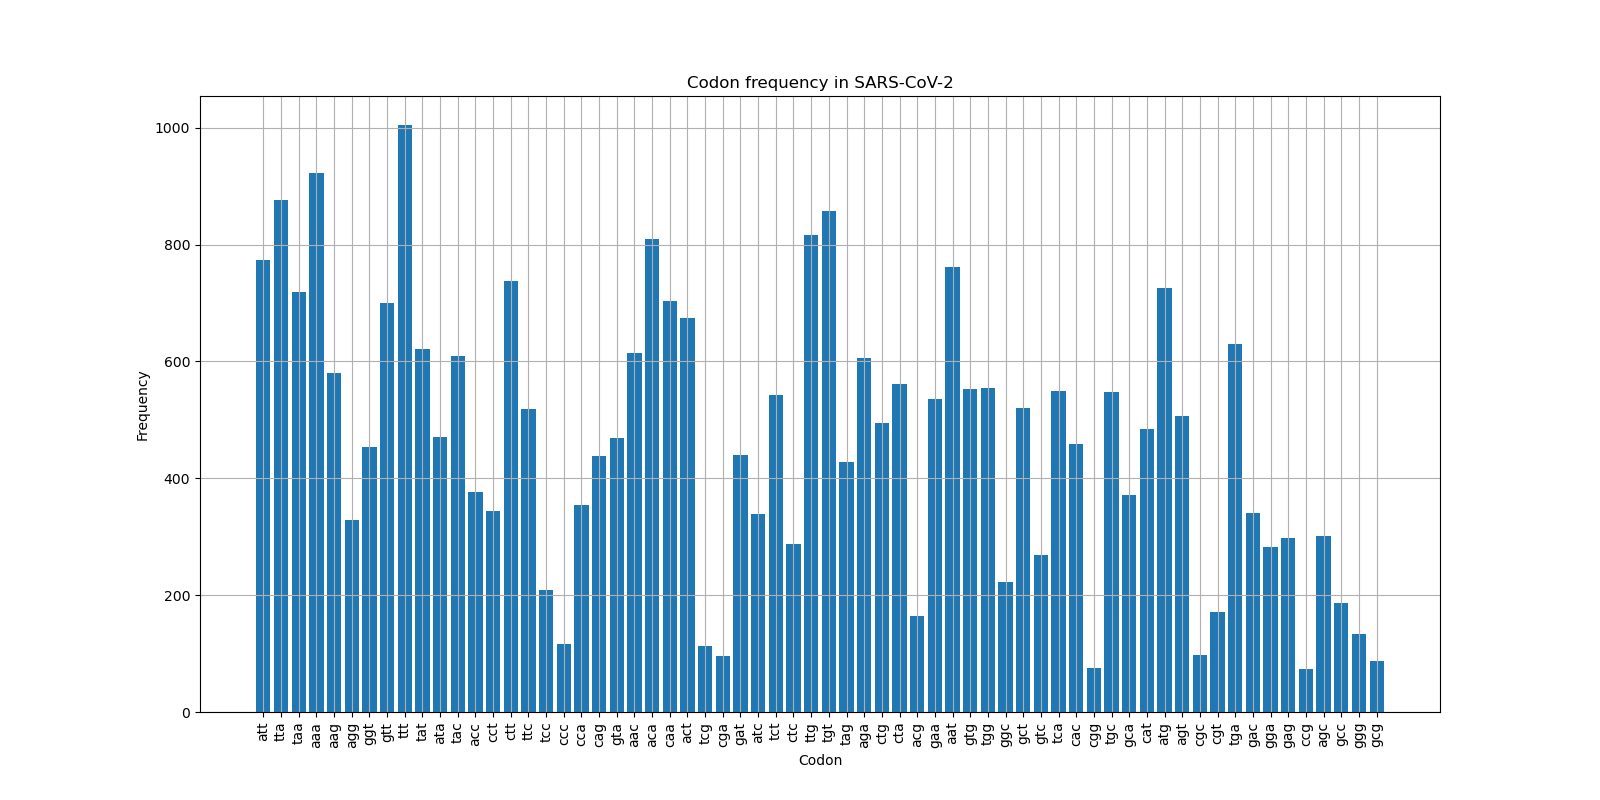
\includegraphics{histogram}
    \caption{\textbf{histogram of codons}}
\end{figure}

\begin{thebibliography}{1}

\bibitem{covid} CDC \emph{COVID-19} https://www.cdc.gov/coronavirus/2019-ncov/index.html

\end{thebibliography}
